%2multibyte Version: 5.50.0.2953 CodePage: 1252

\documentclass[bigger]{beamer}
%%%%%%%%%%%%%%%%%%%%%%%%%%%%%%%%%%%%%%%%%%%%%%%%%%%%%%%%%%%%%%%%%%%%%%%%%%%%%%%%%%%%%%%%%%%%%%%%%%%%%%%%%%%%%%%%%%%%%%%%%%%%%%%%%%%%%%%%%%%%%%%%%%%%%%%%%%%%%%%%%%%%%%%%%%%%%%%%%%%%%%%%%%%%%%%%%%%%%%%%%%%%%%%%%%%%%%%%%%%%%%%%%%%%%%%%%%%%%%%%%%%%%%%%%%%%
\usepackage{amssymb}
\usepackage{amsfonts}
\usepackage{amsmath}
\usepackage{mathpazo}
\usepackage{hyperref}
\usepackage{graphicx}
%\usepackage{multimedia}

%\setcounter{MaxMatrixCols}{10}
%TCIDATA{OutputFilter=LATEX.DLL}
%TCIDATA{Version=5.50.0.2953}
%TCIDATA{Codepage=1252}
%TCIDATA{<META NAME="SaveForMode" CONTENT="1">}
%TCIDATA{BibliographyScheme=Manual}
%TCIDATA{Created=Monday, October 27, 2008 15:56:24}
%TCIDATA{LastRevised=Friday, February 05, 2016 11:57:14}
%TCIDATA{<META NAME="GraphicsSave" CONTENT="32">}
%TCIDATA{<META NAME="DocumentShell" CONTENT="Other Documents\SW\Slides - Beamer">}
%TCIDATA{Language=American English}
%TCIDATA{CSTFile=beamer.cst}

%\newenvironment{stepenumerate}{\begin{enumerate}[<+->]}{\end{enumerate}}
%\newenvironment{stepitemize}{\begin{itemize}[<+->]}{\end{itemize} }
%\newenvironment{stepenumeratewithalert}{\begin{enumerate}[<+-| alert@+>]}{\end{enumerate}}
%\newenvironment{stepitemizewithalert}{\begin{itemize}[<+-| alert@+>]}{\end{itemize} }
\usetheme{Madrid}
\usecolortheme{beaver}
\usefonttheme{professionalfonts}
\input{tcilatex}
\setbeamertemplate{navigation symbols}{}
\begin{document}

\title[47-809: Function Approximation]{Function Approximation}
\subtitle{Judd Chapter 6}
\author[David Childers]{David Childers (thanks to Y. Kryukov, K. Judd, and U. Doraszelski)}
\institute[CMU]{CMU, Tepper School of Business}
\date[Mar.27-29]{Mar 27-29, 2023}
\maketitle

%TCIMACRO{\TeXButton{BeginFrame}{\begin{frame}}}%
%BeginExpansion
\begin{frame}%
%EndExpansion

\frametitle{The Plan}

\begin{itemize}
\item Motivation

\item Local approximations; Taylor, Pade, logs



\item Interpolation
\begin{itemize}
\item Polynomials
\item Splines
\end{itemize}

\item Next Class: More Global Methods 

\begin{itemize}
\item Projection and Regression

\item Orthogonal basis functions

\item Multi-dimensional approaches
\end{itemize}



\end{itemize}


\end{frame}%

\begin{frame}%
%EndExpansion
\frametitle{Motivation, example 1}

Bellman's functional equation:%
\begin{equation*}
V\left( k\right) =\max_{k^{\prime }\geq 0}\pi \left( k\right) +\beta V\left(
k^{\prime }\right)
\end{equation*}

\begin{itemize}
\item Want to find $V\left( \cdot \right) $, e.g. via fixed-point iteration:%
\begin{equation}
V^{k+1}\left( k\right) =\max_{k^{\prime }\geq 0}\pi \left( k\right) +\beta
V^{k}\left( k^{\prime }\right)  \tag{*}
\end{equation}

\item To find max, we need $V^{k}\left( k^{\prime }\right) $ or its
derivative, at any $k^{\prime }$

\begin{itemize}
\item We need a differentiable approximation $\hat{V}\left( \cdot \right) $
\end{itemize}

\item Don't want to compute exact $V^{k}\left( k\right) $ for too many
values of $k$

\begin{itemize}
\item Instead, use them to construct the approximation
\end{itemize}
\end{itemize}

%TCIMACRO{\TeXButton{EndFrame}{\end{frame}}}%
%BeginExpansion
\end{frame}%
%EndExpansion
%TCIMACRO{\TeXButton{BeginFrame}{\begin{frame}}}%
%BeginExpansion
\begin{frame}%
%EndExpansion
\frametitle{Motivation, example 2}

\begin{itemize}
\item Have utility function $u(x_{1},x_{2})$, want Demand for good 1

\item Need to find $D_{1}(p_{1})=D(p_{1},\bar{p}_{2})$, where 
\begin{eqnarray}
D(p) &=&\arg \max u(x_{1},x_{2})  \TCItag{**} \\
\text{subject to} &\text{:}&p_{1}x_{1}+\bar{p}_{2}x_{2}\leq B  \notag
\end{eqnarray}

\item Will need to evalute $D_{1}(p_{1})$ at many points, \newline
e.g. when integrating for CS, or solving monopolist's problem

\item Want to solve (**) for a few points, and

\begin{itemize}
\item Construct an accurate approximation to $D_{1}(p_{1})$

\item That is easy to integrate or differentiate analytically \newline
(i.e. a polynomial)
\end{itemize}
\end{itemize}

%TCIMACRO{\TeXButton{EndFrame}{\end{frame}}}%
%BeginExpansion
\end{frame}%
%EndExpansion
%TCIMACRO{\TeXButton{BeginFrame}{\begin{frame}}}%
%BeginExpansion
\begin{frame}%
%EndExpansion
\frametitle{Approximation stages}

\begin{enumerate}
\item Choose approach (family $\mathcal{F}_m$ of approximating functions, eg polynomials of degree m)

\item Obtain "data" for estimation

\begin{itemize}

\item Choose $n$ \emph{functionals}: $f_i(y())\in\mathbb{R}$ to evaluate
\item E.g., choose node(s) $x_{i}$ and obtain $y_{i}\equiv y\left( x_{i}\right)$ 
\item Data may also contain derivatives $y^{\prime }\left( x_{i}\right)$ or integrals $\int f_{i}(x)y(x)dx$
\end{itemize}

\item Map data to (representation of) $\hat{y}(.)\in\mathcal{F}_m$ e.g. coefficients

\item Evaluation: plug in any $x$, get back $\hat{y}\left( x\right) $
\end{enumerate}

\begin{itemize}
\item "Approximation" could refer to any of these stages

\item Each stage is repeated more frequently than previous ones
\end{itemize}

%TCIMACRO{\TeXButton{EndFrame}{\end{frame}}}%
%BeginExpansion
\end{frame}%
%EndExpansion
%TCIMACRO{\TeXButton{BeginFrame}{\begin{frame}}}%
%BeginExpansion
\begin{frame}%
%EndExpansion
\frametitle{Local approximation: Taylor series}

\begin{itemize}
\item Degree $n$ Taylor approximation to $f\left( x\right) $ around $x_{0}$: 
\begin{eqnarray*}
t(x) &=&f(x_{0})+f^{\prime }(x_{0})(x-x_{0})+\frac{1}{2}f^{\prime \prime
}(x_{0})(x-x_{0})^{2} \\
&&\quad \quad +\ldots +\frac{1}{n!}f^{(n)}(x_{0})(x-x_{0})^{n}
\end{eqnarray*}

\item Error grows rapidly with $\left\vert x_{0}-x\right\vert $; \newline
declines with $n$ within the \emph{convergence radius }$r$

\item Theorem 6.1.2: $r$ $\leq $ distance to nearest singularity of $f$

\item Singularity: $x$ such that $f^{(n)}(x)=\infty $
\end{itemize}

Example:

\begin{itemize}
\item $f(x)=x^{\frac{1}{3}}$ has a singularity at $x=0$.

\item $\Rightarrow $ Taylor series expansion around $x_{0}=1$ \newline
breaks down outside $[0,2]$
\end{itemize}

%TCIMACRO{\TeXButton{EndFrame}{\end{frame}}}%
%BeginExpansion
\end{frame}%
%EndExpansion
%TCIMACRO{\TeXButton{BeginFrame}{\begin{frame}}}%
%BeginExpansion
\begin{frame}%
%EndExpansion
\frametitle{Taylor approximation around \emph{x} = 1}

% \FRAME{ftbpF}{4.0222in}{2.815in}{0pt}{}{}{taylor.png}{\special{language
% "Scientific Word";type "GRAPHIC";maintain-aspect-ratio TRUE;display
% "ICON";valid_file "F";width 4.0222in;height 2.815in;depth 0pt;original-width
% 3.2197in;original-height 2.2468in;cropleft "0";croptop "1";cropright
% "1";cropbottom "0";filename 'Taylor.PNG';file-properties "XNPEU";}}

\scalebox{0.6}{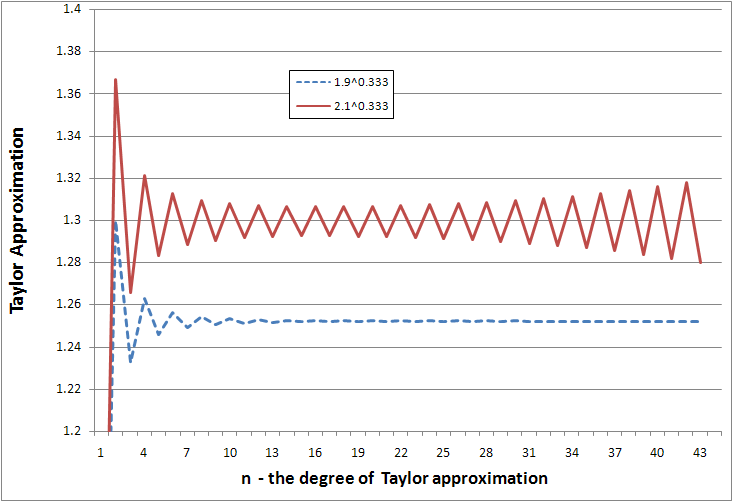
\includegraphics{Taylor.png}}


\end{frame}%

\begin{frame}%

\frametitle{Pade approximation}

\begin{itemize}
\item \emph{Taylor}: polynomial of degree $n$, $%
t^{(i)}(x_{0})=f^{(i)}(x_{0}) $, $i\leq n$

\item \textbf{Pade}: rational function:%
\begin{equation*}
r(x)=p(x)/q(x)
\end{equation*}%
$p(x)$ -- polynomial of degree $n$; $q(x)$ -- of degree $m$

\item Coeff's of $p$ and $q$ -- determined from a system of linear equations:%
\begin{equation*}
\frac{d^{k}}{dx^{k}}(p-f\ast q)(x_{0})=0,\quad k=0,\ldots ,m+n
\end{equation*}

\item More accurate than Taylor, not affected by singularities

\item Read Judd on simplifying the implementation
\end{itemize}

%TCIMACRO{\TeXButton{EndFrame}{\end{frame}}}%
%BeginExpansion
\end{frame}%
%EndExpansion
%TCIMACRO{\TeXButton{BeginFrame}{\begin{frame}}}%
%BeginExpansion
\begin{frame}%
%EndExpansion
\frametitle{Log-Linearization: one example}

Linear approximation to \% deviations (from steady state)

\begin{itemize}
\item Take a production function: $y_{t}=z_{t}k_{t}^{\alpha }$.

\begin{itemize}
\item Take logs: $\ln y_{t}=\ln z_{t}+\alpha \ln k_{t}$
\item Now exactly linear
\end{itemize}

\item To interpret: compare to linearization in levels

\item We know the steady state: $\left( y^{\ast },z^{\ast },k^{\ast }\right) 
$

\begin{itemize}
\item Taylor around it: $\ln y_{t}\approx \ln y^{\ast }+\left( y_{t}-y^{\ast
}\right) /y^{\ast }$

\item Same for $\ln z_{t}$, $\ln k_{t}$
\end{itemize}

\item Plug these into log of production function.\newline
Use $\ln y^{\ast }=\ln z^{\ast }+\alpha \ln k^{\ast }$ to derive:%
\begin{equation*}
\frac{y_{t}-y^{\ast }}{y^{\ast }}\approx \frac{z_{t}-z^{\ast }}{z^{\ast }}%
+\alpha \frac{k_{t}-k^{\ast }}{k^{\ast }}
\end{equation*}
\end{itemize}

%TCIMACRO{\TeXButton{EndFrame}{\end{frame}}}%
%BeginExpansion
\end{frame}%
%EndExpansion
%TCIMACRO{\TeXButton{BeginFrame}{\begin{frame}}}%
%BeginExpansion
\begin{frame}%
%EndExpansion
\frametitle{Log-Linearization: another example}

\begin{itemize}
\item Implicit function: $y\left( x\right) $ defined by $f(y,x)=0$

\item Implicit function theorem:%
\begin{equation*}
\frac{dy}{dx}=-\frac{\partial f/\partial x}{\partial f/\partial y}=-\frac{%
f_{x}}{f_{y}}
\end{equation*}

\item Use the fact that $d\ln x=dx/x$:%
\begin{equation*}
d\ln y=-\frac{x}{y}\frac{f_{x}}{f_{y}}\ast d\ln x
\end{equation*}

\item Approximation:%
\begin{equation*}
\ln y-\ln y_{0}\approx -\frac{x_{0}f_{x}\left( y_{0},x_{0}\right) }{%
y_{0}f_{y}\left( y_{0},x_{0}\right) }\left( \ln x-\ln x_{0}\right)
\end{equation*}
\end{itemize}

%TCIMACRO{\TeXButton{EndFrame}{\end{frame}}}%
%BeginExpansion
\end{frame}%
%EndExpansion
%TCIMACRO{\TeXButton{BeginFrame}{\begin{frame}}}%
%BeginExpansion
\begin{frame}%
%EndExpansion
\frametitle{Example of local methods}

Exercise 6.1: $f(x)=\left( x^{\frac{1}{2}}+1\right) ^{\frac{2}{3}}$, $%
x_{0}=1.$

\begin{itemize}
\item Degree 1 and 2 Taylor series approximation: 
\begin{eqnarray*}
t_{1}(x) &=&{2}^{{\frac{2}{3}}}\left( 1+\tfrac{1}{6}\left( x-1\right)
\right) , \\
t_{2}(x) &=&{2}^{{\frac{2}{3}}}\left( 1+\tfrac{1}{6}\left( x-1\right) -%
\tfrac{7}{144}\left( x-1\right) ^{2}\right) ,
\end{eqnarray*}

\item Pad\'{e} approximation (1,1): 
\begin{equation*}
r(x)={2}^{{\frac{2}{3}}}{\frac{24+11\left( x-1\right) }{24+7(x-1)}}.
\end{equation*}

\item Log-linear approximation ($\ln x_{0}=0$): 
\begin{equation*}
l_{1}(x)={2}^{{\frac{2}{3}}}\left( 1+\tfrac{1}{6}\ln (x)\right)
\end{equation*}
\end{itemize}

\end{frame}%

\begin{frame}%

\frametitle{Local methods: Pros and Cons}

\begin{itemize}

\item Cons: Obvious
\begin{itemize}
\item Limited radius of convergence 
\item Moderate accuracy within radius 
\item Need derivatives, can't handle kinks or discontinuities
\end{itemize}

\item Pros:
\begin{itemize}
\item Linear functional forms allow fast calculations by linear algebra even in extremely high dimensions
\item Can leverage fast first order solutions to solve higher order
\item Huge speed gains, good automated software make this first choice
\item At worst, use for rapid prototyping and good initial guess for global methods
\end{itemize}

\end{itemize}

\end{frame}%

\begin{frame}%

\frametitle{Global methods: introduction}

\textbf{Polynomial approximation}: $f(x)\approx \sum_{j=0}^{m}a_{j}p_{j}(x)=%
\hat{f}(x;a)$

\begin{enumerate}
\item Pick $n$ nodes $x_{i}$, compute $f(x_{i})$

\item Pick coefficients $a$ to minimize $\left\vert f\left( x_{i}\right) -%
\hat{f}\left( x_{i}\right) \right\vert $'s
\end{enumerate}

\begin{itemize}
\item $n=m+1$ -- interpolation, can fit $f(x_{i})$'s exactly

\item $n>m+1$ -- regression, typically least squares

\begin{itemize}
\item Unlike Econometrics, we can pick $x_{i}$'s and $p_{j}(\cdot )$'s
\end{itemize}
\end{itemize}

\textbf{Splines}: piece-wise polynomials (of low degree)

\begin{itemize}
\item split $x$ interval into $\inf x=x_{0}<x_{1}<...<x_{m}=\sup x$

\item On each $\left[ x_{j},x_{j+1}\right] $, $\hat{f}(x)=\hat{f}_{j}(x)$ is
a low-order polynomial.

\item Impose continuity: $\hat{f}_{j-1}(x_{j})=\hat{f}_{j}(x_{j})=f\left(
x_{j}\right) $, \newline
smoothness: $\hat{f}_{j-1}^{\prime }(x_{j})=\hat{f}_{j}^{\prime }(x_{j})$,
etc.
\end{itemize}

%TCIMACRO{\TeXButton{EndFrame}{\end{frame}}}%
%BeginExpansion
\end{frame}%
%EndExpansion
%TCIMACRO{\TeXButton{BeginFrame}{\begin{frame}}}%
%BeginExpansion
\begin{frame}%
%EndExpansion
\frametitle{Polynomial approximation by interpolation}

\begin{itemize}
\item Have 'data': $x_{i},$ $y_{i}=f\left( x_{i}\right) $, $i=1,\ldots ,n$

\item Find a polynomial of degree $n-1$ that satisfies 
\begin{equation*}
p(x_{i})=y_{i},\quad i=1,\ldots ,n.
\end{equation*}

\item $n$ conditions $\Rightarrow $ $n$ linear equations pinning down 
\newline
the $n$ coefficients of $p(\cdot )$:%
\begin{equation*}
a_{0}+a_{1}x_{i}+a_{2}x_{i}^{2}+...+a_{n-1}x_{i}^{n-1}=y_{i},i=1,...,n
\end{equation*}

\item System of linear equations $Va=y$

\item $V$ = Vandermonde matrix, often has large condition number

\item Lots of computation for new $y_{i}$'s (solving $Va=y$); \newline
few computations to evaluate $p\left( x\right) $ for an arbitrary $x$
\item Precompute QR if repeatedly computing coefficients w/ new data at same points
\begin{itemize}
\item $O(n^3)$ overhead for $O(n^2)$ per step
\end{itemize}

\end{itemize}


\end{frame}%

\begin{frame}%

\frametitle{Direct approach: Lagrange interpolation}

\begin{itemize}
\item If coefficients not needed, can avoid computing them completely
\item Explicit solution to $p(x_{i})=y_{i}$ equations: 
\begin{equation*}
p(x)=\sum_{i=1}^{n}y_{i}l_{i}(x),
\end{equation*}%
where 
\begin{equation*}
l_{i}(x)=\prod\nolimits_{j\neq i}\frac{x-x_{j}}{x_{i}-x_{j}}.
\end{equation*}

\begin{itemize}
\item Note that $l_{i}(x_{i})=1$, $l_{i}(x_{j})=0$ if $i\neq j$.
\end{itemize}

\item In practice, do not compute directly: slow and unstable

%\item Lots of computations to evaluate at a new $x$.
%\begin{itemize}
%\item Few computations for a new set of $y_{i}$'s\bigskip
%\end{itemize}

\end{itemize}


\end{frame}

\begin{frame}
\frametitle{Better implementation: Barycentric formula}

\begin{itemize}

\item Use \emph {Barycentric Formula} to find polynomial interpolation
\item Set $p(x_i)=y_i$ and for all other $x$
\begin{equation*}
p(x)=\sum_{i=1}^{n}\frac{\lambda_{i}y_{i}}{x-x_i}/\sum_{i=1}^{n}\frac{\lambda_{i}}{x-x_i}
\end{equation*}%
where 
\begin{equation*}
\lambda_{i}(x)=\frac{1}{\prod\nolimits_{j\neq i}({x_{i}-x_{j}})}.
\end{equation*}

\item $O(n^2)$ to get weights $\lambda_i$, then $O(n)$ per evaluation
\begin{itemize}
\item Same order as if polynomial known even w/ new data $y_i$
\end{itemize}

\item Is polynomial interpolation a good idea? Depends on choice of $x_i$

\end{itemize}

\end{frame}%

\begin{frame}%

\frametitle{Problems with polynomial interpolation}

\scalebox{1.1}{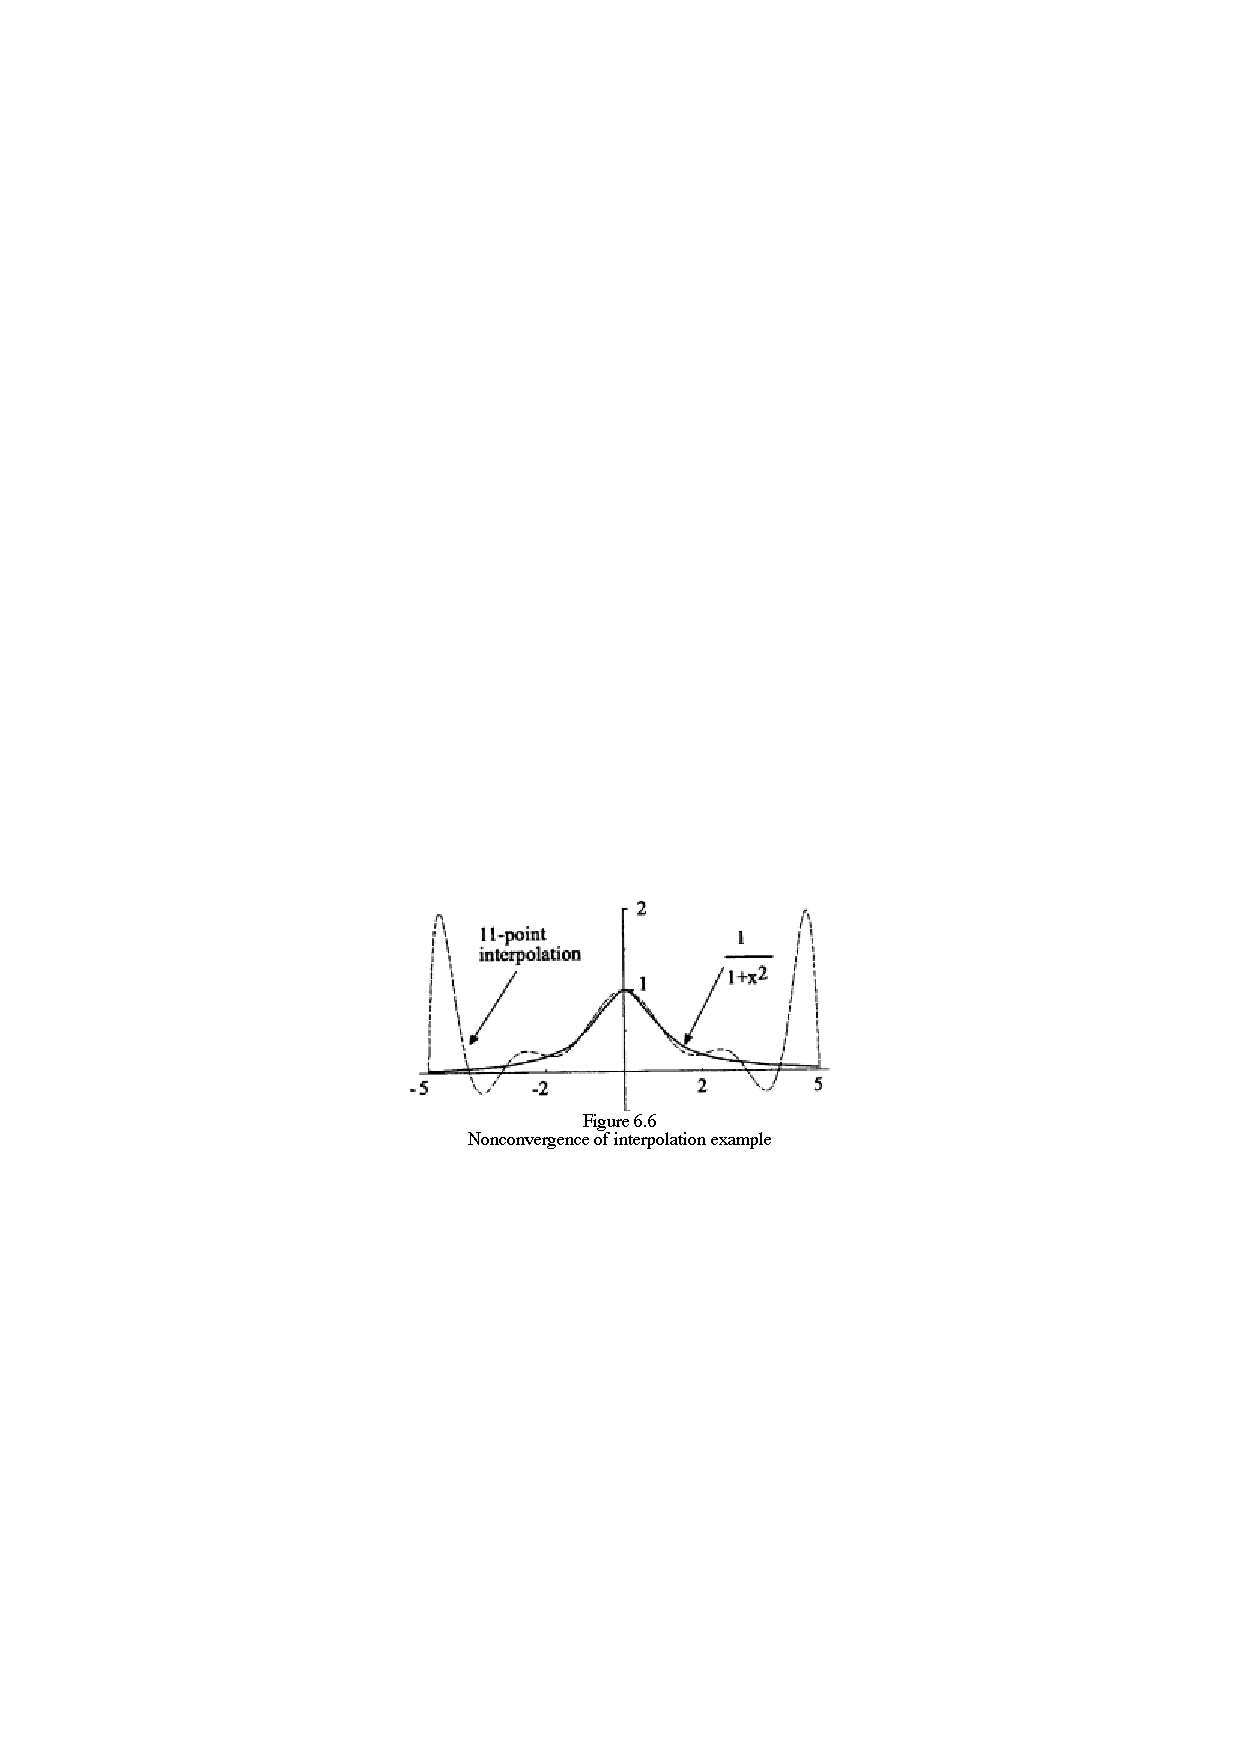
\includegraphics{Fig66Runge.pdf}}
\begin{itemize}

\item Runge Phenomenon: interpolation at evenly spaced points 
\item Interpolation may diverge even if true function $\infty-$differentiable
\item Solution: use stable point set, non-polynomial functions, or projection instead of interpolation
\end{itemize}


\end{frame}%

\begin{frame}%

\frametitle{Possible improvement: Hermite interpolation}

\begin{itemize}
\item Have data: $x_{i}$, $y_{i}=f\left( x_{i}\right) ,$ $y_{i}^{\prime
}=f^{\prime }\left( x_{i}\right) $, $i=1,\ldots ,n$

\item Find a polynomial of degree $2n-1$ that satisfies 
\begin{equation*}
p(x_{i})=y_{i},\quad p^{\prime }(x_{i})=y_{i}^{\prime }\quad i=1,\ldots ,n.
\end{equation*}%
$2n$ conditions $\Rightarrow $ $2n$ linear equations to pin down the $2n$
coefficients of $p$.

\item Explicit solution: 
\begin{equation*}
p(x)=\sum_{i=1}^{n}y_{i}h_{i}(x)+\sum_{i=1}^{n}y_{i}^{\prime }\tilde{h}%
_{i}(x),
\end{equation*}%
where 
\begin{eqnarray*}
\tilde{h}_{i}(x) &=&(x-x_{i})\left[ l_{i}(x)\right] ^{2}, \\
h_{i}(x) &=&(1-2l_{i}^{\prime }(x_{i})(x-x_{i}))\left[ l_{i}(x)\right] ^{2}.
\end{eqnarray*}%
Note $l_{i}^{\prime }(x_{i})=\sum_{j\neq i}\frac{1}{x_{i}-x_{j}}$.
\end{itemize}


\end{frame}%

\begin{frame}%

\frametitle{Major improvement: Good point sets}

\begin{itemize}
\item Optimal point set depends on true and approximating functions, desired convergence class
\item For polynomials on $\left[-1,1\right]$, smooth functions, uniform approximation, near best are Chebyshev points
\begin{equation*}
x_i=\cos(\frac{i\pi}{n})\ \left\{i\in 0 \ldots n\right\} 
\end{equation*}
\item Thm: Let $f(x)$ have $k^{th}$ derivative with total variation $V$ and let $\hat{f}_n(x)$ be interpolation using $n+1$ Chebyshev points
\begin{equation*}
\left\Vert \hat{f}_n(x)-f(x)\right\Vert_{\infty}\leq \frac{4V}{\pi k (n-k)^k} 
\end{equation*}
\item Many other desirable computational properties: next class 

\end{itemize}


\end{frame}%

\begin{frame}%
%EndExpansion
\frametitle{Alternative for general point sets: Splines}

A function $s(x)$ on $[a,b]$ is a spline if:

\begin{itemize}
\item There is a grid of points (nodes or knots)\newline
$a=x_{0}<x_{1}<\ldots <x_{n-1}<x_{n}=b$, ...

\item ... such that $s(x)$ is a polynomial of degree $k$ \newline
on each subinterval $[x_{i-1},x_{i}]$, $i=1,2,\ldots ,n$, ...

\item ... and $s(x)\in \mathbf{C}^{k-1}$ (continuously differentiable to $%
k-1 $ order)

\item Order of the spline can be defined as $k$ or $k+1\bigskip $

\item Linear spline: Piecewise linear, "connecting the
dots.\textquotedblright\ 

\item Cubic spline: $s(x)=a_{i}+b_{i}x+c_{i}x^{2}+d_{i}x^{3}$. $\bigskip $

\item Low cost of computation: efficient sparse matrix algorithms

\item Rapid convergence when $\left\vert x_{i-1}-x_{i}\right\vert
\rightarrow 0$ \newline
rate = $k-1$ if $f\in \mathbf{C}^{k-1}$

\item Good for functions that are not $\mathbf{C}^{\infty }$
\end{itemize}

%TCIMACRO{\TeXButton{EndFrame}{\end{frame}}}%
%BeginExpansion
\end{frame}%

\begin{frame}%

\frametitle{Example: cubic spline}

$s(x)=a_{i}+b_{i}x+c_{i}x^{2}+d_{i}x^{3}$ on $[x_{i-1},x_{i}]$.

\begin{itemize}
\item $2n$ interpolation conditions: 
\begin{eqnarray*}
y_{i} &=&a_{i}+b_{i}x_{i}+c_{i}x_{i}^{2}+d_{i}x_{i}^{3},\quad i=1,\ldots ,n,
\\
y_{i} &=&a_{i+1}+b_{i+1}x_{i}+c_{i+1}x_{i}^{2}+d_{i+1}x_{i}^{3},\quad
i=0,\ldots ,n-1,
\end{eqnarray*}

\item $2n-2$ derivative conditions:%
\begin{eqnarray*}
b_{i}+2c_{i}x_{i}+3d_{i}x_{i}^{2}
&=&b_{i+1}+2c_{i+1}x_{i}+3d_{i+1}x_{i}^{2}, i=1,\ldots,n-1, \\
2c_{i}+6d_{i}x_{i} &=&2c_{i+1}+6d_{i+1}x_{i},\quad i=1,\ldots ,n-1.
\end{eqnarray*}

\item Need 2 end conditions. E.g., the secant Hermite spline:%
\begin{equation*}
s^{\prime }(x_{0})=\frac{y_{1}-y_{0}}{x_{1}-x_{0}},\quad s^{\prime }(x_{n})=%
\frac{y_{n}-y_{n-1}}{x_{n}-x_{n-1}},
\end{equation*}

\item $4n$ linear equations identify the $4n$ coefficients of $s$.
\end{itemize}


\end{frame}%

\begin{frame}%

\frametitle{More splines}

B-splines (de Boor (1978)): good for deriving analytical results about other splines

\begin{itemize}
\item A basis of orthogonal functions

\item Each function is non-zero over two adjacent intervals

\item Recursive formulation $\Rightarrow $ increasing smoothness\bigskip
\end{itemize}

Shape-preserving splines:

\begin{itemize}
\item Concave data might lead to non-concave spline

\item Schumaker procedure

\item Intermediate nodes $z_{i}\in \lbrack x_{i-1},x_{i}]$, data on $%
f^{\prime }(x_{i})$
\end{itemize}


\end{frame}%



\begin{frame}%

\frametitle{Recap of approximations}

\begin{itemize}
\item Want $f\left( x\right) $ for many different $x$'s

\begin{itemize}
\item $f\left( \cdot \right) $ takes a long time to evaluate

\item $\Rightarrow $ use approximation $\hat{f}\left( x\right)
=\sum_{k=0}^{m}a_{k}p_{k}(x)$
\end{itemize}

\item Want to find $a_{k}$ with as little data as possible:

\begin{itemize}
\item Local around $x_{0}$: $f\left( x_{0}\right) $, $f^{\prime }\left(
x_{0}\right) $, $f^{\prime \prime }\left( x_{0}\right) $, ..., $f^{\left(
n\right) }\left( x_{0}\right) $

\item Global: $f\left( x_{1}\right) $, $f\left( x_{2}\right) $, ..., $%
f\left( x_{n}\right) $
\end{itemize}

\item Similar to prediction in Econometrics

\begin{itemize}
\item But econometrics uses observational data

\item Here, we can "design the experiment"
\end{itemize}

\item Smart choice of polynomials $p_{k}(\cdot )$ and nodes $x_{i}$.
\end{itemize}


\end{frame}%

\begin{frame}

\frametitle{Basis Function Methods}

\begin{itemize}

\item Represent function by finite set of coefficients on known set of functions $\phi_k()$

\item Approximation: $p(x)=\sum_{k=0}^{n}a_{k}\phi _{k}(x)$

\item \textbf{Mean Square} ($L^{2}$) approximation: 
\begin{equation*}
\min_{a}\int \left[ f(x)-p(x)\right] ^{2}w(x)dx\Leftrightarrow
\min_{a}\left\Vert f-p\right\Vert _{2}
\end{equation*}

\item \textbf{Uniform} ($L^{\infty }$) approximation: 
\begin{equation*}
\min_{a}\sup_{x}\left\vert f(x)-p(x)\right\vert \Leftrightarrow
\min_{a}\left\Vert f-p\right\Vert _{\infty }
\end{equation*}

\item Usually don't target optimal uniform approximation directly \newline
For many classes (Chebyshev, B-spline, Wavelet, Fourier), good $L^2$ approx implies good $L^\infty$ 

\item \textbf{Derivatives} may not converge
\end{itemize}


\end{frame}%




\begin{frame}%

\frametitle{Orthogonal bases}

\begin{itemize}

\item  Define ($w(x)$ weighted) inner product:%
\begin{equation*}
\left\langle f,g\right\rangle =\int f(x)g(x)w(x)dx.
\end{equation*}

\item The family of functions $\{\phi _{k}\}$ is \textbf{mutually
orthogonal} \newline
iff $\ \left\langle \phi _{k},\phi _{m}\right\rangle =0$ for all $k\neq m$.

\begin{itemize}
\item They \emph{span a subspace} within the space of functions
\end{itemize}

\item Optimal $L^2$ approximation has simple formula when $\phi_k$ \emph{orthogonal} 
\begin{itemize}
\item $a_{k}^{\ast }=\dfrac{<f,\phi _{k}>}{<\phi _{k},\phi _{k}>}$
\item Can calculate separately by direct computation of integral
\end{itemize}

\item Orthogonality also leads to better conditioning when regression approach used


\end{itemize}


\end{frame}%


\begin{frame}%

\frametitle{Why orthonormality?}

\begin{itemize}

\item Complete orthonormal basis gives mean square representation
\item \emph{Parseval's theorem}: 
\begin{itemize}
\item Let $\left\Vert f \right\Vert_{2}^{2}:= \int f(x)^2w(x)dx<\infty$ and $\left\{\phi_{k}\right\}_{k=1}^{\infty}$ be a complete o.n.b. Then
\begin{equation*}
\left\Vert\sum_{k=1}^{N}\left\langle f,\phi_{k}\right\rangle\phi_{k}-f\right\Vert_{2}^{2}=\sum_{k=N+1}^{\infty}a_k^2
\end{equation*}
\end{itemize}
\item Allows representation of continuum by countable family
\begin{itemize}
\item and good, \emph{quantifiable} approximation by finite family
\end{itemize}
\item $L^2$ good enough for some things
\begin{itemize}
\item Integrals, some functional equations, \emph{not} pointwise convergence
\end{itemize}
\item Compare Weierstrass's theorem: Let $f$ continuous, then $\underset{p_N}{\inf}\underset{x}{\sup}|f(x)-p_N(x)|\to 0$
\item Fine, but no speed results, sequence may depend on (unknown) f



\end{itemize}


\end{frame}%

\begin{frame}

\frametitle{From convergence to rates}


\begin{itemize}

\item When does projection representation ensure pointwise convergence?
\item Function must live in strict subset of $L^2$
\item Many many classes exist, usually "smoothness conditions"
\begin{itemize}
\item $\mathcal{C}^k$ k-times continuously differentiable, 
\item Sobolev: $W^{p,k}:=\left\{f:\left\Vert \frac{d^k}{dx}f(x)\right\Vert_p<\infty\right\}$
\item Holder: $\Lambda^\alpha:=\left\{f:\underset{x,y}{\sup}|\frac{d^{\left\lfloor a\right\rfloor}}{dx}f(y)-\frac{d^{\left\lfloor a\right\rfloor}}{dx}f(x)|\leq Cd(x,y)^{a-\left\lfloor a\right\rfloor}\right\}$
\item See also: Besov, Bounded Variation, Reproducing Kernel Hilbert Spaces, etc
\end{itemize} 
\item Each class admits rates in some norms for some basis set
\item Technique: demonstrate class membership by analytical methods (eg map preserves derivatives or integrals, etc)
\item Then use suitable basis given class knowledge
\end{itemize}


\end{frame}%


\begin{frame}%

\frametitle{Orthogonal families}

\begin{tabular}{lccl}
\textbf{Family} & $w(x)$ & \textbf{Domain} & \textbf{definition} \\ \hline
Legendre & $1$ & $[-1,1]$ & $P_{n}(x)=\frac{(-1)^{n}}{2^{n}n!}\frac{d^{n}}{%
dx^{n}}\left( (1-x^{2})^{n}\right) $ \\ 
Chebyshev & $(1-x^{2})^{-\frac{1}{2}}$ & $[-1,1]$ & $T_{n}(x)=\cos \left(
n\cos ^{-1}(x)\right) $ \\ 
Laguerre & $e^{-x}$ & $[0,\infty )$ & $L_{n}(x)=\frac{e^{x}}{n!}\frac{d^{n}}{%
x^{n}}\left( x^{n}e^{-x}\right) $ \\ 
Hermite & $e^{-x^{2}}$ & $(-\infty ,\infty )$ & $H_{n}(x)=(-1)^{n}e^{x^{2}}%
\frac{d^{n}}{dx^{n}}\left( e^{-x^{2}}\right) $ \\ 
Fourier & 1 & $[-\pi ,\pi ]$ & $\frac{1}{2};\cos (nx);\sin (mx)$ \\
Wavelet & 1 & $[-1,1]$ & No closed form \\%
\end{tabular}

\begin{itemize}
\item Look for domain and shape that fits your application

\item Chebyshev is a common choice in Economics

\item Fourier is used for periodic functions, rare in Econ

\item Useful polynomial families have recurrence formulas:

\begin{itemize}
\item $\phi _{0}(x)=1$, $\qquad \phi _{1}(x)=x$

\item $\phi _{k+1}(x)=\left[ c_{k+1}x+d_{k+1}\right] \phi
_{k}(x)+e_{k+1}\phi _{k-1}(x)$
\end{itemize}

\end{itemize}


\end{frame}%

\begin{frame}%

\frametitle{Details: Legendre}

\scalebox{1.7}{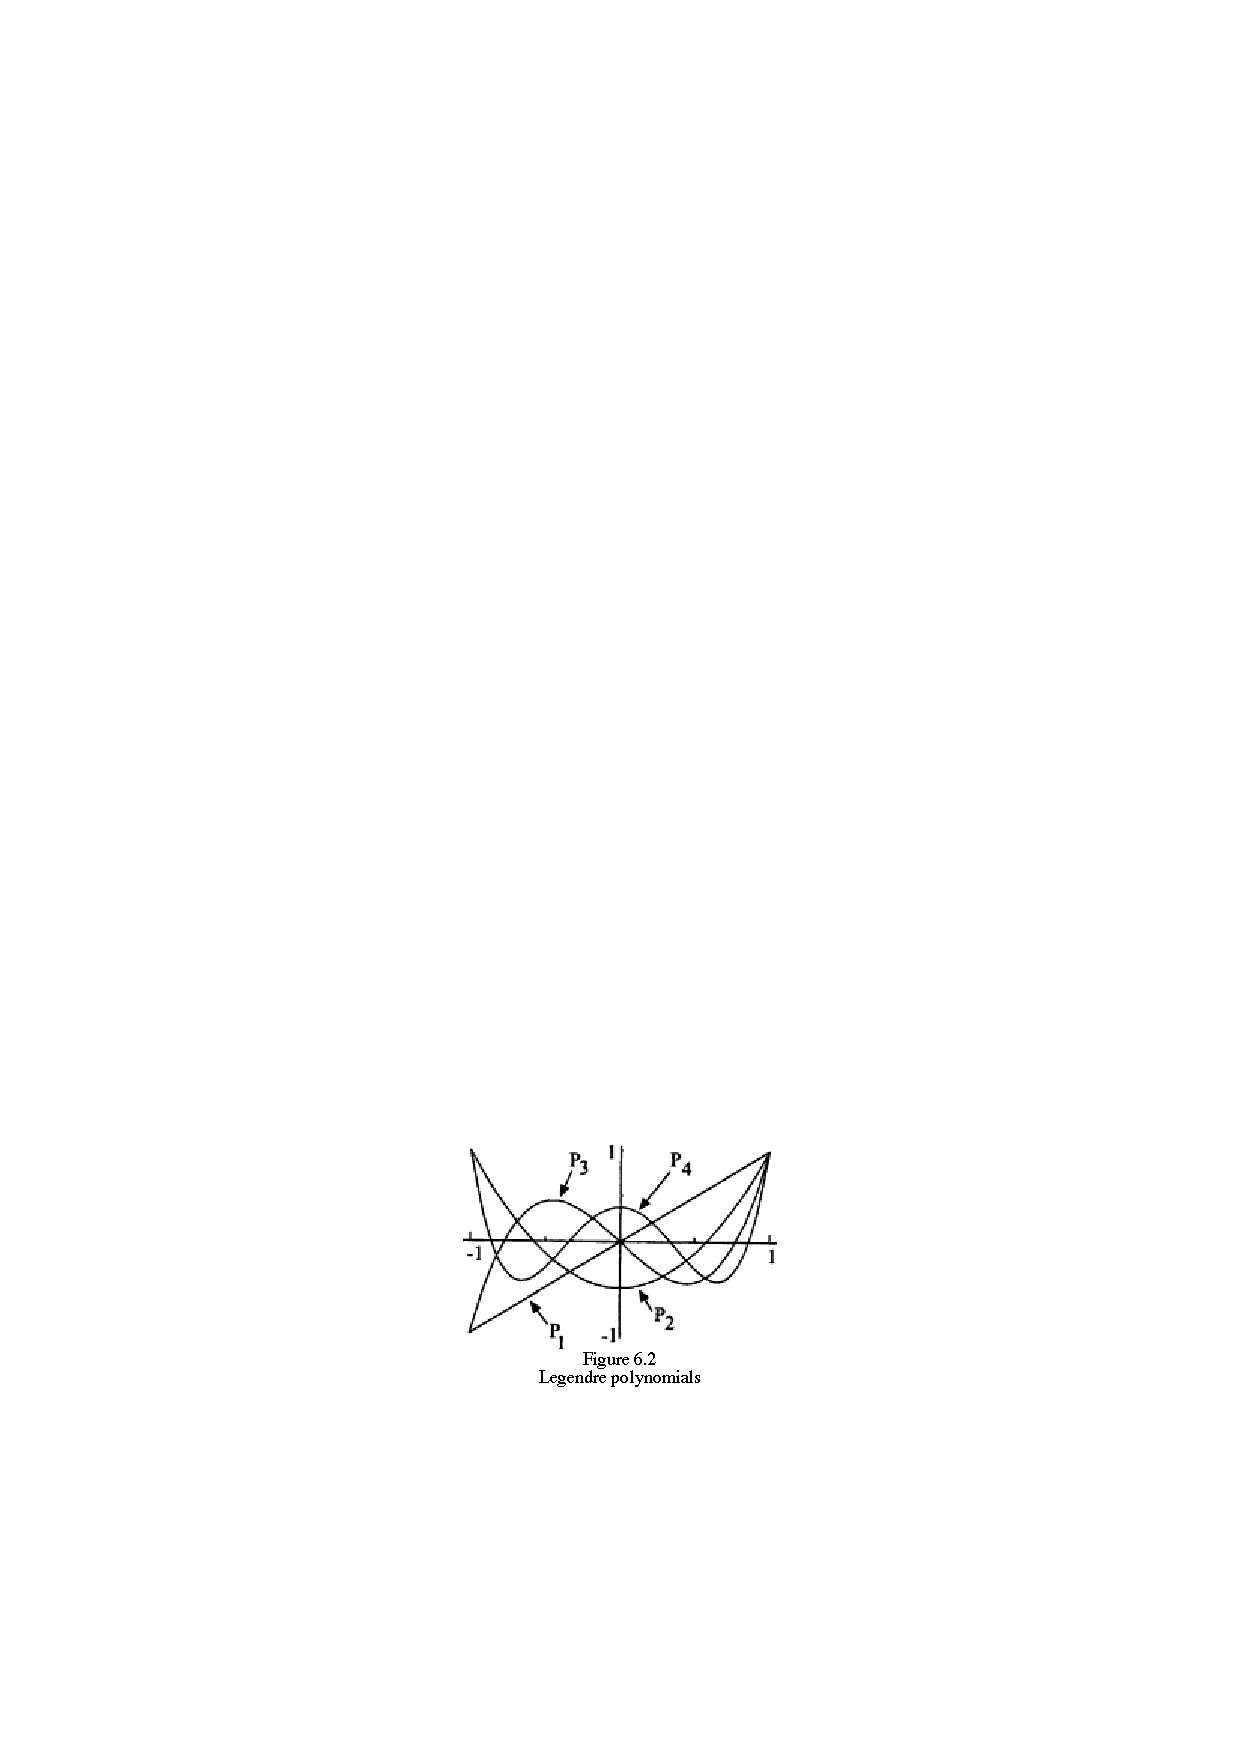
\includegraphics{Fig62Legendre.pdf}}


\end{frame}%

\begin{frame}%
%EndExpansion
\frametitle{Details: Chebyshev}

\scalebox{1.7}{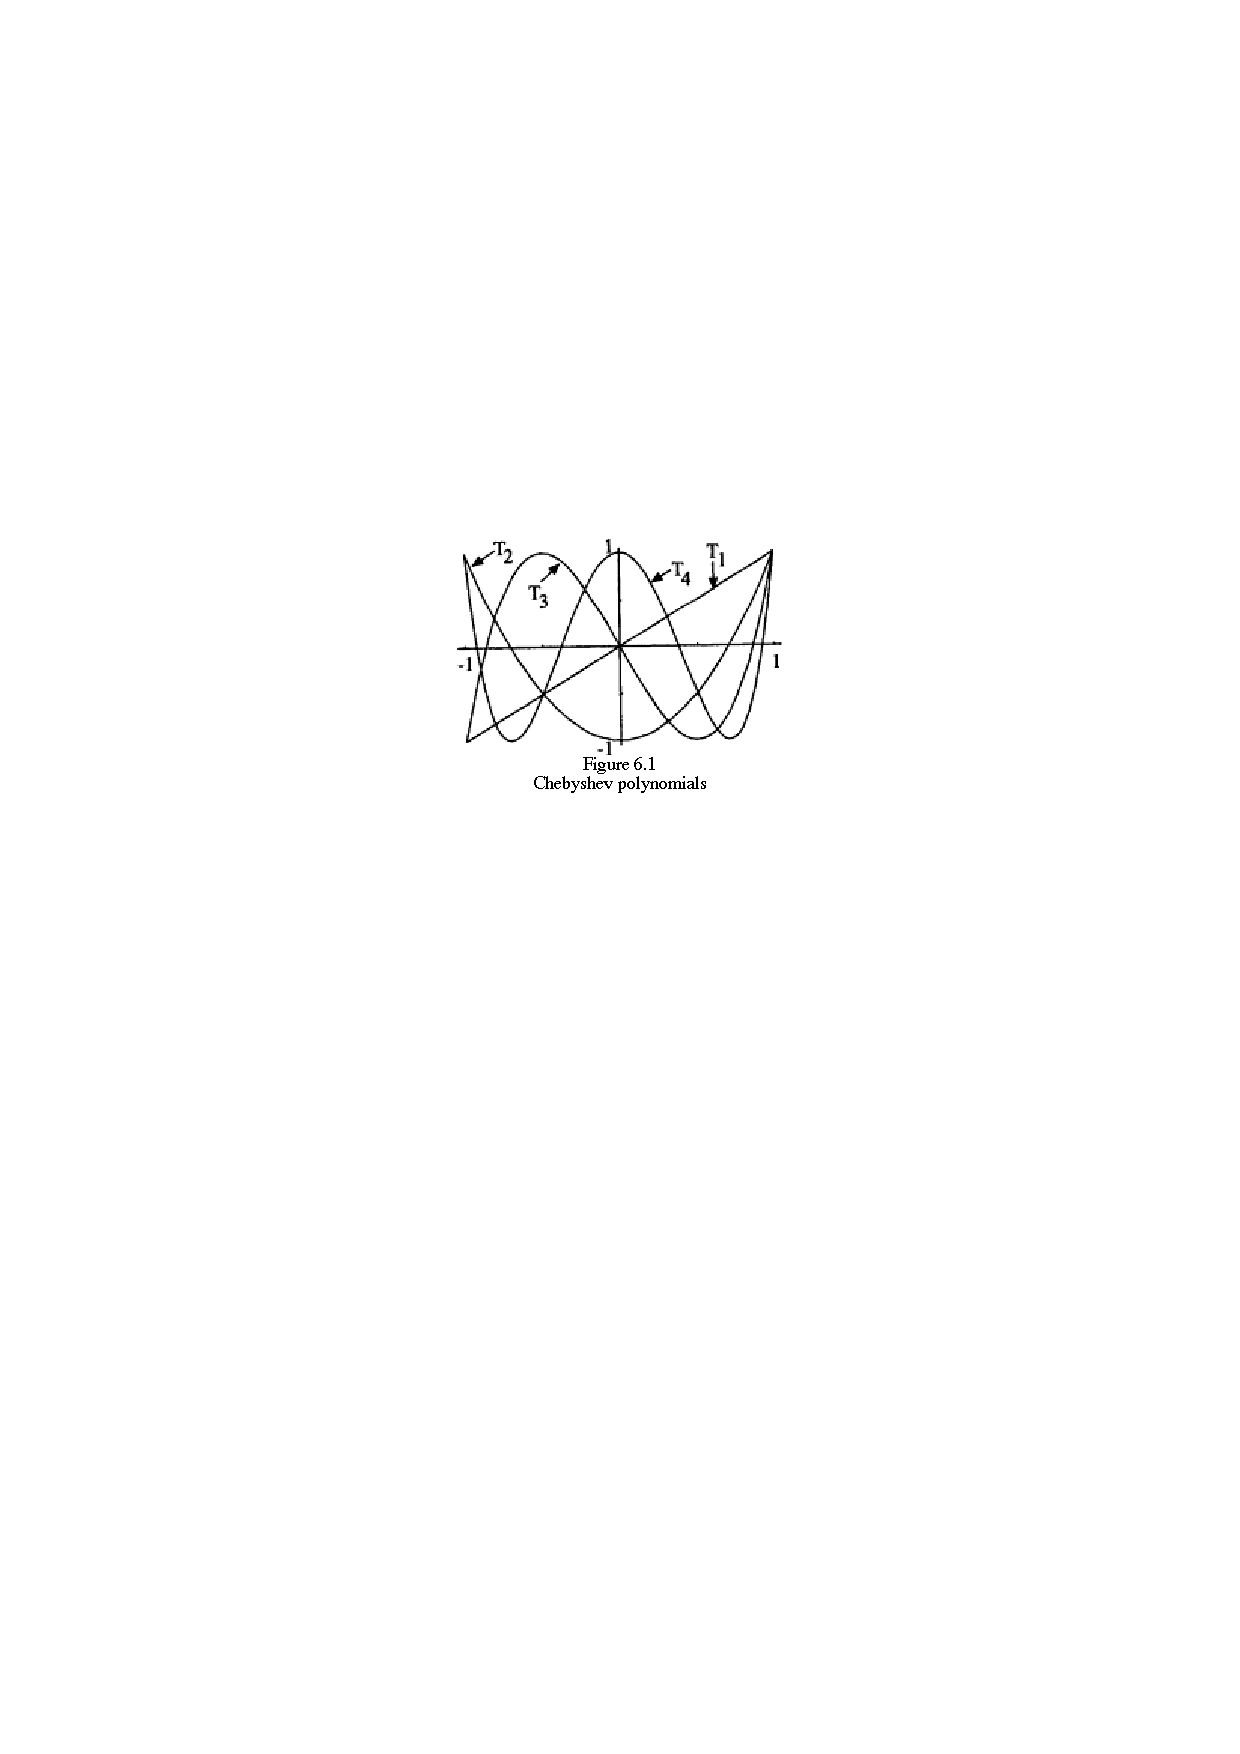
\includegraphics{Fig61Chebyshev.pdf}}



\end{frame}%

\begin{frame}%

\frametitle{Details: Laguerre}

\scalebox{1.7}{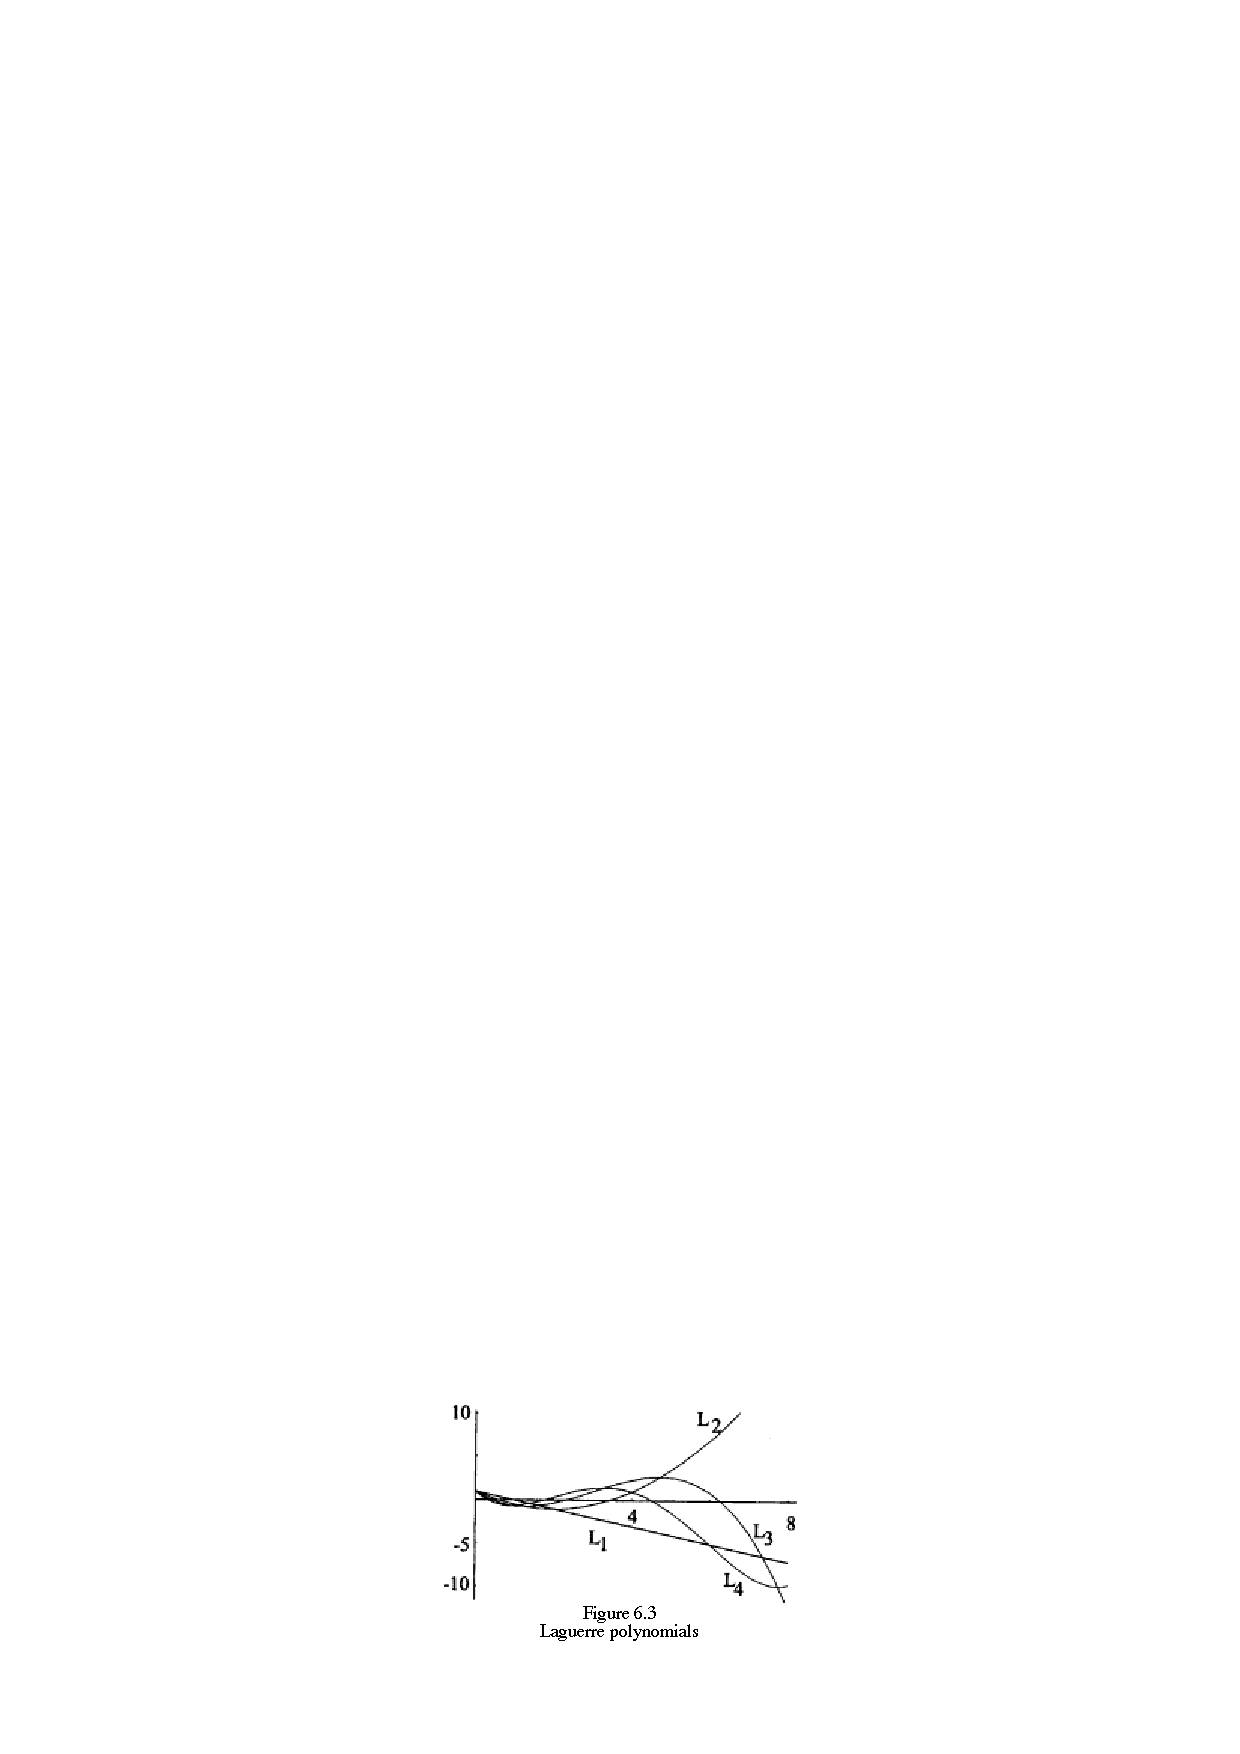
\includegraphics{Fig63Laguerre.pdf}}



\end{frame}%

\begin{frame}%

\frametitle{Details: Hermite}

\scalebox{1.7}{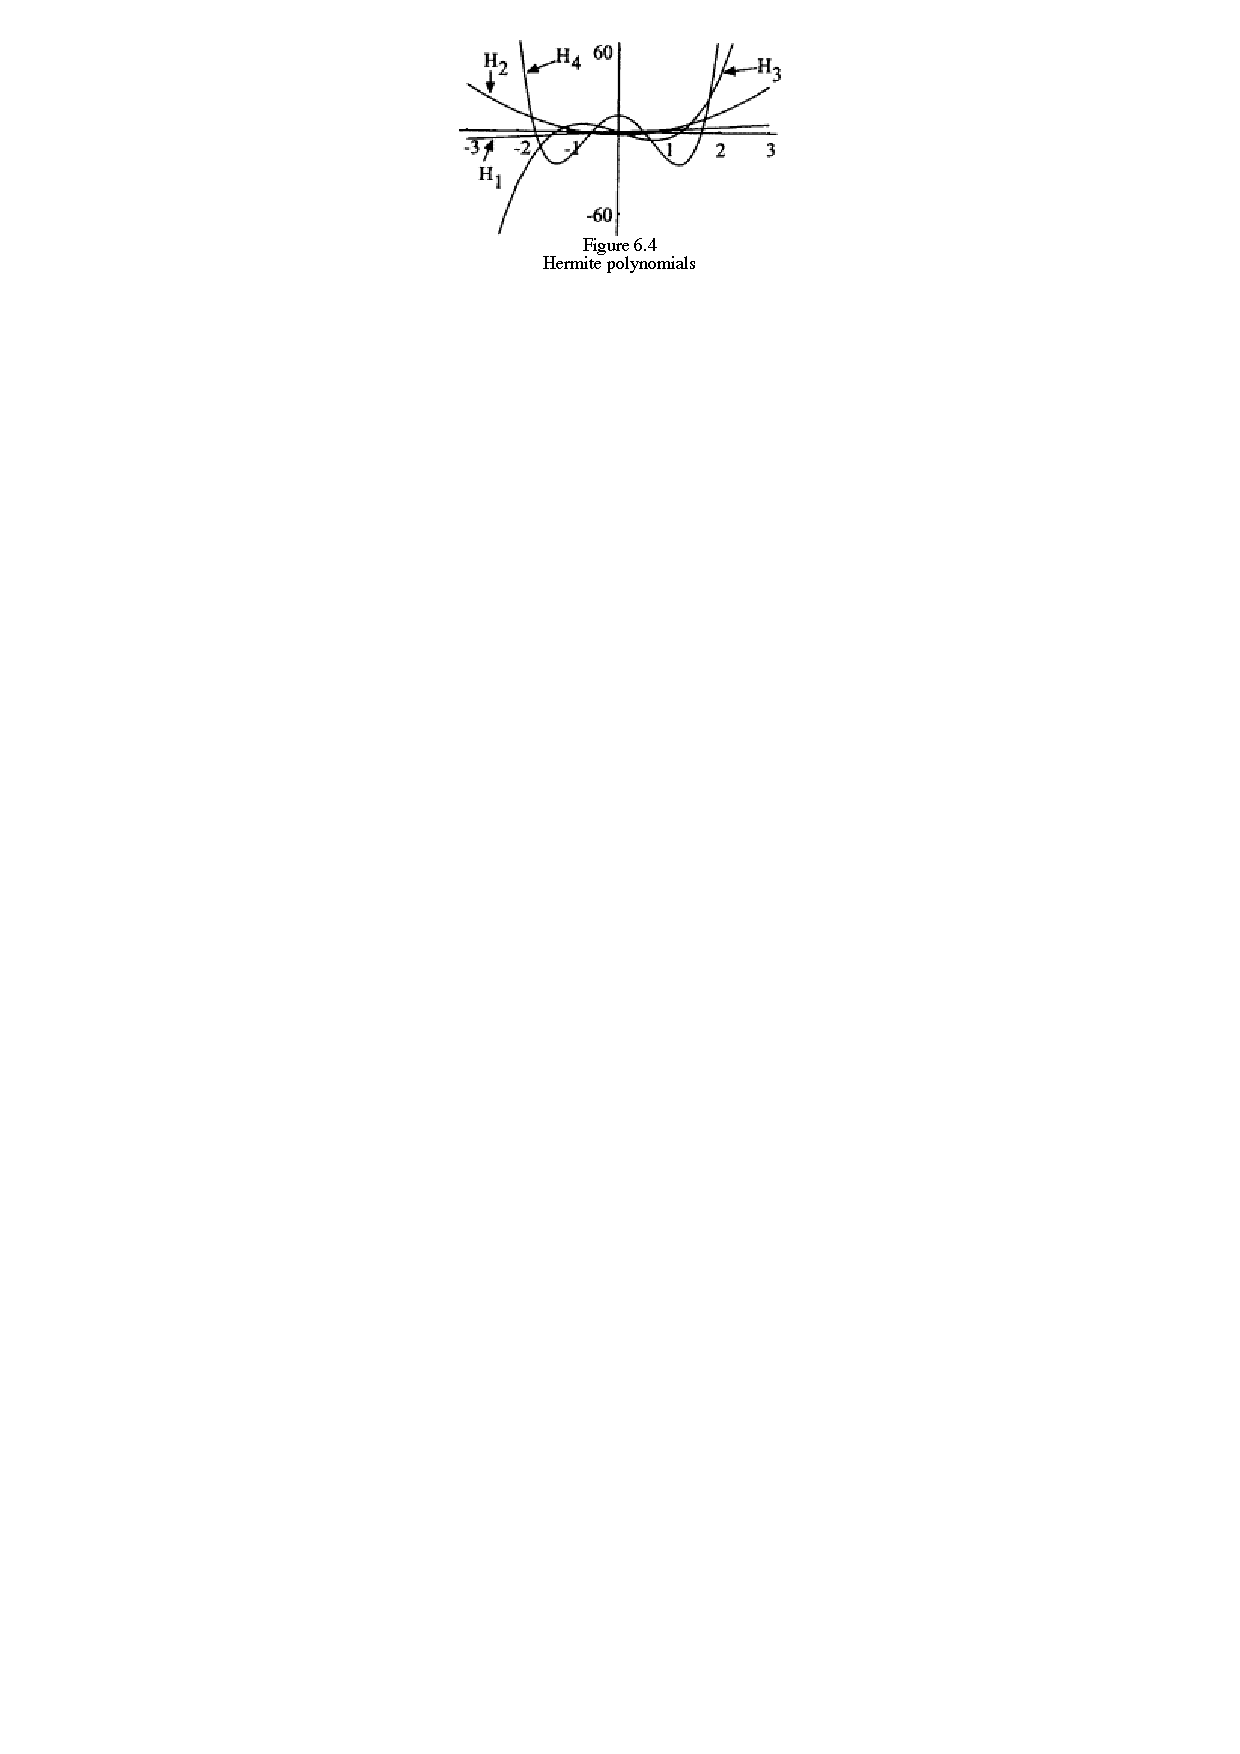
\includegraphics{Fig64Hermite.pdf}}



\end{frame}%



% \begin{frame}%
% %EndExpansion
% \frametitle{Another example: Bernstein polynomials}
% 
% \begin{itemize}
% \item Definition: $B_{i,n}\left( x\right) =\left( \QATOP{n}{i}\right)
% x^{i}\left( 1-x\right) ^{n-i}$,
% 
% \begin{itemize}
% \item where: $x\in \left[ 0,1\right] $, $i=0,...,n$
% 
% \item Recursive formula does not speed up computation
% \end{itemize}
% 
% \item Approximation:%
% \begin{equation*}
% \hat{f}_{n}\left( x\right) =\tsum\nolimits_{i=0}^{n}f\left( i/n\right)
% B_{i,n}\left( x\right)
% \end{equation*}
% 
% \item If $B_{i,n}\left( x\right) \geq 0\Rightarrow \hat{f}_{n}\left(
% x\right) \geq 0$: pdf, policy \& value functions, etc.
% 
% \item Allow for multiple peaks
% 
% \item As $n\rightarrow \infty $:
% 
% \begin{itemize}
% \item $\hat{f}_{n}\rightarrow f$ \textbf{uniformly}
% 
% \item $\hat{f}_{n}^{\prime }\rightarrow f^{\prime }$, also uniformly
% \end{itemize}
% \end{itemize}
% 
% 
% \end{frame}%



\begin{frame}%

\frametitle{Regression Approach to Finding Coefficients}

\begin{enumerate}
\item \textbf{Set-up} (at beginning of code):

\begin{enumerate}
\item Choose functions $\phi \left( \cdot \right) $, order $n$, and \# of
nodes $m\geq n+1$

\item Select nodes $z_{k}$ in the function's support, $k=1,...,m$:\newline
polynomial zeros, or just a uniform grid

\item Map each $z_{k}$ into $x_{k}$ in the support of the target function

\item Evaluate function $\phi _{j}\left( z_{k}\right) $, $j=0,...,n$; 
\newline
store them as a matrix $X:X_{kj}=\left\{ \phi _{j}\left( z_{k}\right)
\right\} $
\end{enumerate}

\item \textbf{Estimation} of coefficients $a=\left[ a_{0},...,a_{m}\right] $:

\begin{enumerate}
\item Evaluate $y_{k}=f\left( x_{k}\right) $; form them into vector $Y$

\item If $m=n+1$, solve $Xa=Y$

\item If $m>n+1$, solve $\left( X^{\prime }X\right) a=X^{\prime }Y$
\end{enumerate}

\item \textbf{Evaluation} of $\hat{f}\left( \bar{x}\right) $ an for an
arbitrary $\bar{x}$

\begin{enumerate}
\item Map $\bar{x}$ into $\bar{z}$ (i.e. into the support of $\phi $)

\item Compute $\phi _{j}\left( \bar{z}\right) $'s; recursive formula will
save time

\item Compute $\hat{f}\left( \bar{x}\right) =\sum_{j=0}^{n}a_{j}\phi
_{j}\left( \bar{z}\right) $
\end{enumerate}
\end{enumerate}


\end{frame}%


\begin{frame}%

\frametitle{Properties of regression approach}

\begin{itemize}

\item When $m=n$, this is just interpolation: \newline
accurate for Chebyshev on Chebyshev points (or Fourier on uniform grid), not otherwise
\item In both cases, interpolation system solved in $n\log(n)$ time by \emph{Fast Fourier Transform}

\item Choose $n>>m$ for general case to converge to projection coefficients

\item Accuracy of order $n$ projection depends on $f$ and $\left\{\phi\right\}$
\item For polynomials: Jackson and Bernstein inequalities: 
\begin{equation*}
\underset{p_n}{\inf}\left\vert f-p_n \right\vert \leq Cn^{-(k+a)}
\end{equation*}
holds iff $f$ has $k$ derivatives which are $a$-Holder-continuous
\item Use theory to derive properties, pick suitable class

\end{itemize}

\end{frame}%


\begin{frame}%

\frametitle{Changing (bounded) domain}

Linear change of variable preserves orthogonality:

\begin{itemize}
\item $\left[ a,b\right] $ to $\left[ -1,1\right] $: $z=-1+2\tfrac{x-a}{b-a}$

\item $\left[ a,+\infty \right] $ to $\left[ 0,+\infty \right] $: $\frac{1}{%
\lambda }\left( x-a\right) $

\begin{itemize}
\item $\lambda $ helps match the area of curvature of the polynomial $%
\bigskip $
\end{itemize}
\end{itemize}

Other useful transformations:

\begin{itemize}
\item $\left( -\infty ,+\infty \right) $ to $\,(0,+\infty )$: $e^{x}$

\item $\left( 0,+\infty \right) $ to $\left( -\infty ,+\infty \right) $: $%
\ln x$

\item $\left( -\infty ,+\infty \right) $ to $\left[ 0,1\right] $: $%
1/(e^{-x}+1)$ = the logistic function

\item $\left[ 0,1\right] $ to $\left( -\infty ,+\infty \right) $: inverted
logistic function
\end{itemize}


\end{frame}%

\begin{frame}%

\frametitle{Changing unbounded domain}

\begin{itemize}
\item Laguerre: $[0,\infty )$. Hermite: $\left( -\infty ,+\infty \right) $

\item Math will work without change of domain

\item But polynomials have curvature and extrema \newline
concentrated in a neighborhood of $0$

\begin{itemize}
\item E.g. Laguerre deg. 4 no extrema outside $\left[ 0,10\right] $
\end{itemize}

\item If $f\left( x\right) $ has most curvature happening on $\left[ 0,\bar{X%
}\right] $,\newline
it might make sense to rescale: $z=x\left( 10/\bar{X}\right) $

\item You can experiment with rescaling to obtain the best fit
\end{itemize}


\end{frame}



% \begin{frame}%
% 
% \frametitle{Chebyshev regression}
% 
% Approximating $f(x)$ on $[a,b]$, degree $n$, $m\geq n+1$ nodes
% 
% \begin{enumerate}
% \item Compute $m$ nodes of interpolation: 
% \begin{equation*}
% z_{k}=-\cos \left( \frac{2k-1}{2m}\pi \right) ,\quad k=1,\ldots ,m.
% \end{equation*}
% 
% \item Map into $[a,b]$: $x_{k}=(z_{k}+1)\left( \frac{b-a}{2}\right) +a$, $%
% k=1,\ldots ,m$.
% 
% \item Evaluate $f$ at the nodes: $y_{k}=f(x_{k})$, $k=1,\ldots ,m$.
% 
% \item Given choice of nodes, the optimal coefficients are: 
% \begin{equation*}
% c_{i}=\dfrac{\sum_{k=1}^{m}y_{k}T_{i}(z_{k})}{\sum_{k=1}^{m}T_{i}(z_{k})^{2}}%
% \quad i=0,\ldots ,n
% \end{equation*}
% \end{enumerate}
% 
% $\Rightarrow $ Approximation: $C_{n}(x)=\sum_{i=0}^{n}c_{i}T_{i}\left( 2%
% \frac{x-a}{b-a}-1\right) $.
% 
% 
% \end{frame}%
% 
% \begin{frame}%
% 
% \frametitle{More on Chebyshev regression}
% 
% \begin{itemize}
% \item The $m$ nodes, are zeros of a degree $m$ Chebyshev polynomial
% 
% \begin{itemize}
% \item Coefficient formula depends on these nodes
% 
% \item Can use other nodes with regular OLS formula:\newline
% $\left( T^{\prime }T\right) ^{-1}T^{\prime }y$
% \end{itemize}
% 
% \item If $m=n+1$, this is called Chebyshev interpolation
% 
% \item $||f(x)-C_{n}(x)||_{\infty }$ ($L^{\infty }$ norm) converges almost as
% fast \newline
% as the min-max approximation %Quantify!!! Add slide with rates
% %Also, add slide with efficient computation: interpolation formula by FFT is O(nlog(n))
% %Lose higher order factor accuracy relative to projection, which is L^2 optimal, and within log(n) of $L^\infty$ optimal
% 
% \item If $f\in \mathbf{C}^{k}[a,b]$, then there is a constant $\bar{c}$ such
% that 
% \begin{equation*}
% |c_{j}|\leq \frac{\bar{c}}{j^{k}},\quad j\geq 1,
% \end{equation*}%
% i.e., higher-order terms are less relevant
% \end{itemize}
% 
% %In case $f$ is $\mathbf{C}^{\infty}$ or analytic, decay rate exponential
% \end{frame}%

\begin{frame}%

\frametitle{Nonlinear regression approach}

\begin{itemize}
\item Nothing in principle requires using sum of basis functions
\item Can choose nonlinear class, find parameters by nonlinear least squares
\item Adaptive regression splines: choose knot points and coefficients
\item Neural networks: repeatedly compose linear and nonlinear maps
\begin{itemize}
\item Single \emph{neuron} $j$ is $F_j(\sum_{k=1}^{n}x_{jk}\beta_{jk})$ for pointwise nonlinear function like $F(x)=\max(x,0)$ or logit(x) with inputs $x_{jk}$ and weights $\beta_{jk}$
\item A set of neurons form a \emph{layer}, and are used as inputs to another set of neurons
\end{itemize}
\item Optimization problem harder, so choose only if nonlinear class gives much better approx of true function
\begin{itemize}
\item Adaptive splines improve rates for Bounded Variation functions
\item Neural nets perform well for high-dimensional, irregular functions: space of images, sounds, text
\end{itemize}

\end{itemize}

\end{frame}%

\begin{frame}%

\frametitle{Adaptive methods}

\begin{enumerate}
\item Start with initial grid, 
\item Use one of above methods to approximate 
\item Pick new points, compare approximation and truth
\item Increase order of approximation based on errors
\end{enumerate}

\begin{itemize}
\item Especially useful if easy to refine: e.g. splines, wavelets
\item Alternative: penalized or thresholded approximation
\begin{itemize}
\item Find coefficients, then remove small ones
\item or use procedure that gives only small set of coefs (eg LASSO)
\end{itemize}
\item Result: much smaller set of coefficients
\begin{itemize}
\item Useful if next step has costs depending on number
\end{itemize}
\item Accuracy cost low if true function \emph{sparse} in basis
\begin{itemize}
\item Only a few (knots, wavelets etc) matter: 
\item True if function has small set of spikes/inflections
\item E.g. Models with hard constraints can give sharp breaks
\end{itemize}

\end{itemize}



\end{frame}%

\begin{frame}%

\frametitle{Wavelets}

\begin{itemize}
\item Bespoke basis functions designed for fast optimal approximation
\item Start with pair $\phi(x)$ $\psi(x)$ father and mother wavelet (or scaling function and wavelet)
\item Scaling function self-similar: $\phi(x)=\sum_{k=1}^{n}a_k\phi(2x-k)$
\item Wavelet $\psi(x)=\sum_{k=1}^{m}b_k\phi(2x-k)$
\item $\{\phi_{j,k}(x)=2^{-j/2}\phi(2^{-j}x-k)\}$ $\{\psi_{j,k}(x)=2^{-j/2}\psi(2^{-j}x-k)\}$ are basis collection
\item $n$ coefs calculated recursively in $O(n)$ time by cascade algorithm
\item Can choose so compactly supported, orthogonal, approximate smooth/nonsmooth functions
\item In adaptive methods, use only large coefs $\to$ good approx if function has nonsmooth area, like edge
\item Many families available for different applications
\end{itemize}

\end{frame}%




\begin{frame}%
%EndExpansion
\frametitle{Multi-dimensional approximation}

$F(x):\mathbb{R}^{m}\rightarrow \mathbb{R}$ 

\begin{itemize}
\item \emph{Lagrange interpolation} -- requires careful choice of nodes

\begin{itemize}
\item Otherwise, coefficient equations can become singular
\end{itemize}

\item \emph{Tensor products} of orth. functions in each $x_{i}$
\begin{equation*}
\{\phi_k(x_1)\}_{k=0}^{n}\otimes\{\psi_j(x_2)\}_{j=0}^{n}:=\{\{\phi_k(x_1)\psi_j(x_2)\}_{j=0}^{n}\}_{k=0}^{n}
\end{equation*}

\begin{itemize}
\item Curse of dimensionality: $n^{m}$ coefficients
\end{itemize}

\item \emph{Complete polynomials}: $\sum_{i=1}^{n}j_{i}\leq m$

\begin{itemize}
\item less coefficients, same precision
\end{itemize}

\item \emph{Neural networks}: split function into lower-dimensional ones:%
\newline
$F(x_{1},x_{2},x_{3},x_{4})=\tilde{F}(\tilde{f}_{1}(x_{1},x_{2}),\tilde{f}%
_{2}(x_{3},x_{4}))$

\item Machine Learning methods: Gaussian Process $\&$ RKHS, etc

\end{itemize}


\end{frame}%


\begin{frame}%

\frametitle{Sparse grids approach}


\begin{itemize}

\item If multidimensional function has many cross-partial derivatives

\begin{equation*}
\left\Vert\frac{\partial^{\bar{\alpha}}}{dx_1\ldots dx_m}f(.)\right\Vert<\infty
\end{equation*}
for $\bar{\alpha}=\alpha_1\ldots\alpha_m$ with $\underset{j\in 1\ldots m}{\sup}\alpha_j<k$

\item Then interactions are "not too strong"
\item Can use many fewer grid points away from axes when interpolating than, e.g., tensor product Chebyshev
\item Can efficiently construct \emph{Sparse grids} for interpolation which yield accurate approximation with only polynomial, not exponential dependence on dimension
\item Result is \emph{Smolyak} polynomial (or spline) approximation

\end{itemize}


\end{frame}%


\begin{frame}%

\frametitle{Reproducing Kernel Hilbert Spaces}


\begin{itemize}

\item Complete normed space $\mathcal{H}_K$ of functions $F:\mathcal{X}\to\mathbb{R}$ with inner product $\left\langle,\right\rangle_K$, in which norm convergence implies pointwise convergence
\item Has \emph{reproducing kernel} $k(s,t):\mathcal{X}\times\mathcal{X}\to\mathbb{R}$ s.t. $f(s)=\left\langle f(.),k(s,.)\right\rangle_K$
\item Different $k$ define functions of different shapes, smoothness 
\begin{itemize}
\item "Gaussian kernel" $k(s,t)=C\exp(-\frac{d(s,t)^2}{2\sigma^2})$
\item Defined for any metric space $\mathcal{X}$
\item Good for high-dimensional or strange spaces 
\item $\mathcal{X}$ can be images, text, other functions, etc
\item Smoothing splines: $\mathcal{H}_K=\mathcal{W}^{2,2k}$ $\left\langle f,f\right\rangle_K=\int (f^{\prime\prime})^{2}(x)dx$
\end{itemize}



\end{itemize}


\end{frame}%

\begin{frame}%

\frametitle{Reproducing Kernel Hilbert Spaces: smoothing}


\begin{itemize}

\item Optimal regression $\underset{f\in\mathcal{H}_K}{\inf}(\sum_{i=1}^{m}(y_i-f(x_i))^2+C\left\langle f,f\right\rangle_K)$ 
\begin{itemize}
\item Solution $f=\sum_{i=1}^{m}a_ik(x_i,.)$ where $a_i$ have simple expression
\end{itemize}
\item Cost is $O(m^3)$, independent of dimension of $\mathcal{X}$
\begin{itemize}
\item Can be improved in some cases
\item If $\mathcal{H}_K$ is smoothing splines, get HP filter
\end{itemize}
\item Equivalent to posterior mean of \emph{Gaussian Process} prior
\begin{itemize}
\item  Using data $(y_i,x_i)$ and Gaussian likelihood
\end{itemize}
\item This is prior over functions $f(x)$ where marginals $(f(x_i),f(x_2),\ldots, f(x_n))\sim N(0,K)$
\item $[K]_{ij}:=K(x_i,x_j)$  kernel function is covariance matrix of process
\item Bayesian interpretation: best guess of function given data
\item Also allows calculating uncertainty in approximation

\end{itemize}


\end{frame}%

\begin{frame}%

\frametitle{Python tools}

\begin{itemize}
\item \texttt{scipy.interpolate} offers variety of spline methods

\begin{itemize}
\item Linear: \texttt{numpy.interp}, \texttt{CubicSpline}, B-splines: \texttt{make}$\_$\texttt{interp}$\_$\texttt{spline}, 

\item Also monotone, 2D, N-D spline on regular, irregular grids

\end{itemize}

\item \href{https://github.com/chebpy/chebpy}{chebpy} or \href{https://github.com/pychebfun/pychebfun}{pychebfun}: tools for efficient computation with polynomial and basis methods and applications
\begin{itemize}
\item Treat functions as objects, w/ adaptive Chebyshev representations 
\end{itemize}

\item Specialized libraries for GPs: \href{https://gpytorch.ai/}{GPyTorch}, \href{https://scikit-learn.org/stable/modules/gaussian_process.html}{sklearn.} \href{https://scikit-learn.org/stable/modules/gaussian_process.html}{gaussian}$\_$\href{https://scikit-learn.org/stable/modules/gaussian_process.html}{process}, Signal Processing and Wavelets: \texttt{scipy.signal}, \href{https://github.com/EconForge/Smolyak}{Smolyak}, etc 

\item To learn, read help and try to replicate with your own code

\item You can use these in your research, but not in PS3
\end{itemize}


\end{frame}%

\begin{frame}%

\frametitle{Julia tools}

\begin{itemize}
\item \texttt{interpolate()} in \href{https://github.com/JuliaMath/Interpolations.jl}{\texttt{Interpolations.jl}}

\begin{itemize}
\item Piecewise constant, linear, quadratic, cubic spline

\item Fast on even grids: use other libraries for alternative splines

\item See \href{https://julia.quantecon.org/more_julia/general_packages.html}{QuantEcon} for code examples

\end{itemize}

\item \href{https://github.com/JuliaApproximation/ApproxFun.jl}{ApproxFun} system has huge set of tools for efficient computation with polynomial and basis methods and applications
\begin{itemize}
\item Treats functions as objects, w/ adaptive Chebyshev representations 
\end{itemize}

\item \href{https://github.com/JuliaDSP/Wavelets.jl}{Wavelets.jl}, other specialized packages for \href{https://github.com/STOR-i/GaussianProcesses.jl}{GPs}, \href{https://github.com/RJDennis/SmolyakApprox.jl}{Smolyak}, etc 

\item To learn, read help and try to replicate with your own code

\item You can use these in your research, but not in PS3
\end{itemize}


\end{frame}%

\begin{frame}%

\frametitle{Matlab tools}

\begin{itemize}
\item \texttt{interp1(), interp2(), interpn()}

\begin{itemize}
\item Piecewise constant, linear, or cubic spline

\item Combines estimation and evaluation steps\newline
-- very slow
\end{itemize}

\item \texttt{spline()} can save estimated coefficients for later use in
evaluation

\item \emph{CompEcon} has Chebyshev estimation and evaluation tools
\item \href{http://www.chebfun.org/publications/}{Chebfun} system has huge set of tools for efficient computation with Chebyshev methods and applications
\item Wavelet toolbox for wavelets, GPStuff for Gaussian Processes

\item To learn, read help and try to replicate with your own code

\item You can use these in your research, but not in PS3
\end{itemize}


\end{frame}%

\begin{frame}%

\frametitle{References 1}

\begin{itemize}
\item Judd Ch. 6

\item Global Polynomials
\begin{itemize}
\item Trefethen, Lloyd N. \underline{Approximation Theory and Approximation } \underline{Practice} 2013. \url{http://www.chebfun.org/ATAP/}
\item Boyd, John P. \underline{Chebyshev and Fourier Spectral Methods} 2nd ed. Dover, 2000. \url{http://www-personal.umich.edu/~jpboyd/BOOK_Spectral2000.html}
\end{itemize}


\item Taylor Expansion
\begin{itemize}
\item Fernandez-Villaverde, J., Rubio-Ramirez, J.F., $\&$ Schorfheide, F. "Solution and Estimation Methods for DSGE Models" \underline{Handbook of Macroeconomics} Volume 2A, Ch 9. Elsevier, 2016.
\end{itemize}





\end{itemize}


\end{frame}%

\begin{frame}
\frametitle{References, ctd}
\begin{itemize}
\item Spline and RKHS
\begin{itemize}
\item Algorithms and actual code called by Matlab for splines are in:
\item de Boor, Carl. \underline{A Practical Guide to Splines} Rev. Ed. 2001. 
\item Smoothing splines and RKHSs, classic reference:
\item Wahba, Grace. \underline{Spline Models for Observational Data}  1991.
\end{itemize}
\item Gaussian Process methods:
\begin{itemize}
\item Rasmussen, Carl $\&$ Christopher Williams. \underline{Gaussian Processes for Machine Learning} MIT, 2006. \url{http://www.gaussianprocess.org/gpml/}
\end{itemize}
\item Wavelets (and Fourier)
\begin{itemize}
\item Mallat, Stephane. \underline{A Wavelet Tour of Signal Processing: } \underline{The Sparse Way}, 3rd ed. Elsevier, 2009.
\item G. Peyr\'e. \underline{The Numerical Tours of Signal Processing}, 2011. \url{https://www.numerical-tours.com/}
\end{itemize}

\end{itemize}
\end{frame}

%Add slides on: smoothing splines, RKHS, and Bayesian approach
%Maybe say something about GPs
%Add slides on Smolyak and sparse grid methods
%Add slides on wavelets (definition, implementation, applications) 
%Add details on neural networks (definition, backprop, pros and cons)


\end{document}
